% =============================================================================
% CHAPTER 18: EMERGENT TEMPORAL INTERVENTION THEORY
% =============================================================================
%------------------------------------------------------------------------------
% Chapter 18: Emergent Temporal Intervention Theory
%------------------------------------------------------------------------------
% Version: 4.0 (January 2026) - MAJOR REWRITE: Pure Emergent Theory
%
% Purpose: Develop the emergent temporal theory for interventions:
%          1. Journey-Position emerges from 10C Status Quo Vector (EIT-4)
%          2. Effect-Horizon τ emerges from Intervention Vector (EIT-5)
%          3. Phase-Affinity as continuous function α(→I, →S₀)
%
% IMPORTANT: This chapter does NOT introduce discrete types or archetypes.
%            Heuristic clusters (A1-A8) are deferred to Chapter 20.
%
% Primary Appendix: HHH - METHOD-TOOLKIT (Axioms EIT-1 to EIT-5), AW - CORE-STAGE
% Secondary Appendices: V (WHEN), BB (EQUILIBRIA), K (LIT-FEHR)
%
% Prerequisites: Chapter 13 (Journey), Chapter 17 (Intervention Foundations)
% Leads to: Chapter 19 (Segment-Specific), Chapter 20 (Portfolios + Heuristics)
%
% Chapter Type: C (Application)
%------------------------------------------------------------------------------
% =============================================================================

\chapter{Emergent Temporal Intervention Theory}
\label{ch:journey-integrated}

%%%%%%%%%%%%%%%%%%%%%%%%%%%%%%%%%%%%%%%%%%%%%%%%%%%%%%%%%%%%%%%%%%%%%%%%%%%%%%%
% CHAPTER SCOPE BOX
%%%%%%%%%%%%%%%%%%%%%%%%%%%%%%%%%%%%%%%%%%%%%%%%%%%%%%%%%%%%%%%%%%%%%%%%%%%%%%%
\begin{tcolorbox}[
    colback=purple!5!white,
    colframe=purple!75!black,
    title={\textbf{Chapter Scope: Ziel / In-Scope / Out-of-Scope}},
    fonttitle=\bfseries
]

\textbf{Ziel (Objective):}
Apply the EBF framework to phase-type affinity matrix with practical examples and policy implications.

\vspace{0.3cm}
\textbf{In-Scope:}
\begin{itemize}[nosep]
    \item Practical applications of phase-type affinity matrix
    \item Multiple worked examples (≥2)
    \item Policy implications and recommendations
    \item Implementation guidance
\end{itemize}

\vspace{0.3cm}
\textbf{Out-of-Scope (delegiert an Appendices):}
\begin{itemize}[nosep]
    \item Theoretical foundations $\rightarrow$ Foundation chapters
    \item Formal proofs $\rightarrow$ FORMAL appendices
    \item Parameter estimation methods $\rightarrow$ METHOD appendices
\end{itemize}

\end{tcolorbox}



% -----------------------------------------------------------------------------
% QUICK REFERENCE BOX
% -----------------------------------------------------------------------------
\begin{tcolorbox}[colback=blue!5!white, colframe=blue!75!black,
    title=Zentrale Begriffe in diesem Kapitel]
\small
\begin{tabular}{@{}ll@{}}
\textbf{10C Status Quo $\vec{S}_0$} & Aktueller Zustand: $(L, d, \gamma, \Psi, \Theta, A_0, W_0, \varphi_0, \text{Scope})$ \\
\textbf{Interventionsvektor $\vec{I}$} & Punkt im kontinuierlichen Raum $[0,1]^9$ \\
\textbf{Journey-Position $\varphi$} & \textbf{Emergiert} aus $\vec{S}_0$ via $\varphi = h(\vec{S}_0)$ (EIT-4) \\
\textbf{Wirkungs-Horizont $\tau$} & \textbf{Emergiert} aus $\vec{I}$ via $\tau = g(\vec{I})$ (EIT-5) \\
\textbf{Phase-Affinity $\alpha(\vec{I}, \vec{S}_0)$} & Effektivit\"{a}ts-Multiplikator als \textbf{kontinuierliche Funktion} \\
\textbf{Ko-Evolution} & $\vec{S}(t)$ und $\vec{I}(t)$ entwickeln sich gemeinsam \\
\end{tabular}
\end{tcolorbox}

\begin{tcolorbox}[colback=red!5!white, colframe=red!75!black,
    title=\textbf{Wichtig: Keine diskreten Typen in diesem Kapitel}]
Dieses Kapitel arbeitet ausschließlich im \textbf{kontinuierlichen Interventionsraum} $[0,1]^9$.
Discrete ``Typen'' oder ``Archetypen'' (A1--A8) werden \textbf{nicht} eingeführt---sie sind
heuristische Abkürzungen, die erst in Kapitel 20 behandelt werden. Alle Ergebnisse hier
basieren auf dem vollen Vektor $\vec{I}$, nicht auf Cluster-Zuordnungen.
\end{tcolorbox}

% -----------------------------------------------------------------------------
% APPENDIX REFERENCES BOX
% -----------------------------------------------------------------------------
\begin{tcolorbox}[colback=yellow!10!white, colframe=orange!75!black,
    title=Appendix References for This Chapter]

\textbf{Primär (Emergent Intervention Theory):}
\begin{itemize}[nosep]
\item Appendix HHH (METHOD-TOOLKIT) --- \textbf{Axiom EIT-4} (Journey-Emergence), \textbf{Axiom EIT-5} (Horizon-Emergence)
\item Appendix AW (CORE-STAGE) --- Journey-Axiome, $S(t)$ Dynamik, Phasen-Regionen
\end{itemize}

\textbf{Unterstützend:}
\begin{itemize}[nosep]
\item Appendix V (CORE-WHEN): Temporaler Kontext $\Psi_T$, kritische Zeitfenster
\item Appendix BB (FORMAL-EQUILIBRIA): Übergangs-Dynamiken, Tipping Points
\item Appendix K (LIT-FEHR): Experimentelle Evidenz für Interventions-Effekte
\item Appendix BBB (CORE-WHERE): Literatur-basierte Parameterschätzungen
\item Appendix G (REF-GLOSSARY): Begriffsdefinitionen
\end{itemize}
\end{tcolorbox}

% -----------------------------------------------------------------------------
% CROSS-REFERENCE: EMERGE ALGORITHM (Chapter 11, EIT-EMP)
% -----------------------------------------------------------------------------
\begin{tcolorbox}[colback=blue!5!white, colframe=blue!75!black,
    title=\textbf{Cross-Reference: EMERGE Algorithm \& Phase-K* (Chapter 11, 20)}]

Die Phase-Affinity $\alpha(\vec{I}, \vec{S}_0)$ ist ein \textbf{Kernfaktor} im EMERGE-Algorithmus (Kapitel 11, EIT-EMP-2, \textbf{EXC-3 Hybrid}):

\vspace{0.2cm}
\textbf{K*-Formel mit Stage-Adjustment (EXC-3):}
\begin{equation*}
K^* = K_{\text{base}} \cdot f_B + \delta_C + \underbrace{\delta_S}_{\alpha_{BCJ}} + \delta_\gamma + \delta_L
\end{equation*}
\textit{Nur $f_B$ multiplikativ (Veto-Logik); $\delta_S$ additiv.}

\textbf{Phase → K* Mapping (EIT-EMP-2):}
\begin{itemize}[nosep]
\item \textbf{Pre-Aware} ($\varphi < 0.3$): $f_S = 0.7$ → wenige, aber fokussierte Awareness-Interventionen
\item \textbf{Triggered} ($\varphi \in [0.3, 0.5]$): $f_S = 1.2$ → mehr Interventionen, kritisches Fenster
\item \textbf{Action} ($\varphi \in [0.5, 0.8]$): $f_S = 1.0$ → Standard K* (Commitment + Support)
\item \textbf{Maintenance} ($\varphi > 0.8$): $f_S = 0.8$ → fokussiertes Portfolio für Habit-Formation
\end{itemize}

\vspace{0.2cm}
\textbf{Mismatch-Detection:} Wenn $\alpha(\vec{I}, \vec{S}_0) < 0.3$, warnt EMERGE vor Phase-Mismatch.

\vspace{0.2cm}
\textit{Siehe: Chapter 11 §11.20 (EMERGE), Chapter 20 §20.7 (Constraint C7), Appendix IE}
\end{tcolorbox}

% -----------------------------------------------------------------------------
% INTUITION BOX
% -----------------------------------------------------------------------------

\begin{tcolorbox}[colback=yellow!5!white, colframe=yellow!75!black,
    title=Intuition: Thomas und die drei Ärzte]

\textbf{Thomas}, 52, raucht seit 30 Jahren. Drei Ärzte versuchen verschiedene Strategien:

\textbf{Dr.\ Schmidt (Month 1):}
\begin{itemize}[nosep]
\item Zeigt Lungenkrebs-Statistiken, erklärt Risiken detailliert
\item Thomas nickt höflich, ändert nichts
\item \textit{Diagnose:} Thomas ist in Phase 1 (Pre-Awareness) --- er \textit{weiß} die Fakten, aber sie sind nicht \textit{salient}
\item \textit{Problem:} Information-Intervention in Pre-Awareness Phase hat $\alpha_{1,1} = 0.15$
\end{itemize}

\textbf{Dr.\ Müller (Month 6):}
\begin{itemize}[nosep]
\item Fragt: ``Was würde sich ändern, wenn Sie aufhören?''
\item Thomas reflektiert über Enkel, die er aufwachsen sehen will
\item Plötzlich \textit{will} er aufhören --- Trigger-Moment
\item \textit{Diagnose:} Thomas ist jetzt in Phase 2 (Triggered) --- bereit für Commitment
\item \textit{Richtig:} Identitäts-Intervention zum richtigen Zeitpunkt, $\alpha_{5,2} = 0.75$
\end{itemize}

\textbf{Dr.\ Weber (Month 7):}
\begin{itemize}[nosep]
\item Schlägt Quit-Date vor, Thomas unterschreibt Commitment-Card
\item Nikotinpflaster + tägliche Tracking-App
\item Nach 3 Monaten: Nichtraucher
\item \textit{Diagnose:} Korrekte Sequenz: Commitment (Phase 2→3) + Support (Phase 3→4)
\end{itemize}

\textbf{Kern-Einsicht:} Dieselbe Person braucht \textit{verschiedene} Interventionen in verschiedenen Journey-Phasen. Die richtige Intervention zur falschen Zeit ist die falsche Intervention.
\end{tcolorbox}

% -----------------------------------------------------------------------------
% CENTRAL QUESTION BOX
% -----------------------------------------------------------------------------

\begin{tcolorbox}[colback=red!5!white, colframe=red!75!black,
    title=Central Question]
\textbf{Wie emergiert die Journey-Position aus dem 10C Status Quo Vector, wie emergiert der Wirkungs-Horizont aus dem Interventionsvektor --- und wie bestimmt dies die optimale Interventionsstrategie?}
\end{tcolorbox}

% -----------------------------------------------------------------------------
% METHODOLOGICAL NOTE: EXCLUSION PRINCIPLE
% -----------------------------------------------------------------------------
\begin{tcolorbox}[colback=red!5!white, colframe=red!75!black,
    title=\textbf{Methodological Note: The Exclusion Principle (Appendix FRM)}]
\textbf{Following Appendix FRM (LIT-FEHR-METHOD):}

Dieses Kapitel behauptet Phase $\times$ Intervention Interaktionen ($\alpha_{t,\varphi} \neq \alpha_{t,\varphi'}$). Per Exclusion Principle:
\begin{itemize}[nosep]
    \item \textbf{Null-Hypothese $H_0$:} Interventionen wirken phasenunabhängig ($\alpha_{t,\varphi} = \alpha_t$ für alle $\varphi$)
    \item \textbf{Alternative $H_1$:} Phasenspezifische Effektivität existiert ($\alpha_{t,\varphi}$ variiert mit $\varphi$)
    \item \textbf{Empirischer Test:} Commitment-Device in Phase 1 vs.\ Phase 2 (Prochaska \& DiClemente, 1983)
    \item \textbf{Ergebnis:} $H_0$ verworfen ($p < 0.001$); Commitment in Phase 2: $d = 0.8$, in Phase 1: $d = 0.1$
\end{itemize}

\textbf{Wissenschaftlicher Wert:} Das Journey-Intervention Alignment Principle gewinnt Wert, wo phasenspezifische Interventionen messbar besser performen als phasen-neutrale.
\end{tcolorbox}

% -----------------------------------------------------------------------------
% CHAPTER OVERVIEW
% -----------------------------------------------------------------------------

\begin{tcolorbox}[colback=green!5!white, colframe=green!75!black,
    title=Chapter Overview]

\textbf{Verbindung zu Kapitel 17:} Kapitel 17 etabliert den \textbf{kontinuierlichen Interventionsraum} $[0,1]^9$ und die Emergent Intervention Theory (EIT). Dieses Kapitel entwickelt die \textbf{temporale Dimension}: Wie emergieren Journey-Position und Wirkungs-Horizont aus den fundamentalen Vektoren?

\textbf{Kernfragen:}
\begin{itemize}[nosep]
    \item Wie emergiert $\varphi$ (Journey-Position) aus $\vec{S}_0$?
    \item Wie emergiert $\tau$ (Wirkungs-Horizont) aus $\vec{I}$?
    \item Was bestimmt die Phase-Affinity $\alpha(\vec{I}, \vec{S}_0)$?
\end{itemize}

\begin{enumerate}
\item \textbf{Section~\ref{sec:18-emergence}}: Die zwei Emergenzen --- Journey-Position und Wirkungs-Horizont
\item \textbf{Section~\ref{sec:18-affinity}}: Phase-Affinity als kontinuierliche Funktion
\item \textbf{Section~\ref{sec:18-horizon}}: Wirkungs-Horizont --- Sofort, Kurzfristig, Mittelfristig, Langfristig
\item \textbf{Section~\ref{sec:18-dynamics}}: Ko-Evolution von $\vec{S}(t)$ und $\vec{I}(t)$
\item \textbf{Section~\ref{sec:18-sequence}}: Optimale Interventions-Trajektorien
\item \textbf{Section~\ref{sec:18-mismatch}}: Mismatch-Kosten und Timing-Fehler
\item \textbf{Section~\ref{sec:18-examples}}: Worked Examples
\end{enumerate}

\textbf{Weiter zu Kapitel 20:} Heuristische Cluster (A1--A8) für praktische Anwendungen werden erst in Kapitel 20 eingeführt.
\end{tcolorbox}


%%%%%%%%%%%%%%%%%%%%%%%%%%%%%%%%%%%%%%%%%%%%%%%%%%%%%%%%%%%%%%%%%%%%%%%%%%%%%%%
\section{Die Zwei Emergenzen: Journey-Position und Wirkungs-Horizont}
\label{sec:18-emergence}
%%%%%%%%%%%%%%%%%%%%%%%%%%%%%%%%%%%%%%%%%%%%%%%%%%%%%%%%%%%%%%%%%%%%%%%%%%%%%%%

Dieses Kapitel entwickelt zwei fundamentale Emergenzen der Emergent Intervention Theory (EIT):

\begin{enumerate}
\item \textbf{Journey-Position} $\varphi$ emergiert aus dem 10C Status Quo Vector $\vec{S}_0$
\item \textbf{Wirkungs-Horizont} $\tau$ emergiert aus dem Interventionsvektor $\vec{I}$
\end{enumerate}

\subsection{Axiom EIT-4: Journey-Position Emergenz}

\begin{tcolorbox}[colback=blue!5!white, colframe=blue!75!black,
    title=\textbf{Axiom EIT-4: Journey-Position als emergente Eigenschaft (aus Appendix HHH)}]

\textbf{Statement:} Die aktuelle Position in der Behavioral Change Journey \textit{emergiert} aus dem 10C Status Quo Vector:
\begin{equation}
\boxed{\varphi = h(\vec{S}_0) = h(L, d, \gamma_{\text{current}}, \Psi, \Theta, A_0, W_0, \text{Scope})}
\label{eq:18-journey-emergence}
\end{equation}

\textbf{Kern-Einsicht:} Journey-Phasen sind \textbf{Regionen} im 10C Status Quo Raum, keine ontologischen Kategorien. Grenzen sind \textit{fuzzy}.

\end{tcolorbox}

\subsection{Die Emergenz-Funktion $h(\vec{S}_0)$}

Die Journey-Position emergiert primär aus drei 10C-Dimensionen:

\begin{equation}
\varphi \approx h(A_0, W_0, \text{Scope}) = \frac{1}{1 + e^{-k(A_0 \cdot W_0 \cdot f(\text{Scope}) - \theta)}}
\label{eq:18-emergence-function}
\end{equation}

\begin{table}[htbp]
\centering
\caption{Emergenz-Regionen im 10C Status Quo Raum}
\label{tab:18-emergence-regions}
\renewcommand{\arraystretch}{1.4}
\small
\begin{tabular}{@{}lp{6cm}c@{}}
\toprule
\textbf{Region (ca.)} & \textbf{10C Bedingungen} & \textbf{Traditionelle Phase} \\
\midrule
$\varphi \in [0, 0.2)$ & $A_0 < 0.3 \land W_0 < 0.2$ & Pre-Awareness \\
$\varphi \in [0.2, 0.4)$ & $A_0 > 0.5 \land W_0 < 0.4$ & Triggered \\
$\varphi \in [0.4, 0.6)$ & $A_0 > 0.7 \land W_0 > 0.6 \land \text{Scope} \leq L2$ & Action \\
$\varphi \in [0.6, 0.8)$ & $W_0 > 0.8 \land \text{Scope} \geq L2$ & Maintenance \\
$\varphi \in [0.8, 1.0]$ & $W_0 > 0.9 \land \gamma_{\text{habit}} > 0.7$ & Stable \\
\bottomrule
\end{tabular}
\end{table}

\textbf{Wichtig:} Diese Regionen haben \textit{fuzzy} Grenzen. Eine Person mit $(A_0 = 0.55, W_0 = 0.35)$ liegt ``zwischen'' Triggered und Action---im kontinuierlichen Raum ein valider Zustand.

\subsection{Axiom EIT-5: Wirkungs-Horizont Emergenz}

\begin{tcolorbox}[colback=blue!5!white, colframe=blue!75!black,
    title=\textbf{Axiom EIT-5: Wirkungs-Horizont als emergente Eigenschaft (aus Appendix HHH)}]

\textbf{Statement:} Der temporale Wirkungs-Horizont $\tau$ einer Intervention \textit{emergiert} aus dem Interventionsvektor:
\begin{equation}
\boxed{\tau(\vec{I}) = g(I_{\text{HIERARCHY}}, I_{\text{WHO}}, I_{\text{HOW}})}
\label{eq:18-horizon-emergence}
\end{equation}

\end{tcolorbox}

\subsection{Die vier Wirkungs-Horizonte}

\begin{table}[htbp]
\centering
\caption{Emergenz des Wirkungs-Horizonts aus dem Interventionsvektor}
\label{tab:18-horizon-emergence}
\renewcommand{\arraystretch}{1.4}
\small
\begin{tabular}{@{}llcc@{}}
\toprule
\textbf{Horizont} & \textbf{Interventionsvektor-Bedingung} & \textbf{Zeitraum} & \textbf{Beispiel-Interventionen} \\
\midrule
Sofort & $I_{\text{HIERARCHY}} < 0.2$ (L3) & Stunden--Tage & Real-time Feedback, Alerts \\
Kurzfristig & $I_{\text{HIERARCHY}} \in [0.2, 0.4)$ (L2/L3) & Tage--Wochen & Nudges, Defaults \\
Mittelfristig & $I_{\text{HIERARCHY}} \in [0.4, 0.7)$ (L1/L2) & Wochen--Monate & Programme, Kampagnen \\
Langfristig & $I_{\text{HIERARCHY}} > 0.7$ (L0/L1) + $I_{\text{HOW}} > 0.5$ & Monate--Jahre & Policy, Identitätsarbeit \\
\bottomrule
\end{tabular}
\end{table}

\textbf{Kern-Einsicht:} Eine Intervention, die $I_{\text{HOW}}$ (Komplementaritäten) stark verändert, hat automatisch einen längeren Wirkungs-Horizont als eine, die nur $I_{\text{AWARE}}$ (kurzfristige Aufmerksamkeit) betrifft.

\subsection{Psychologische Fundierung}

Jede emergente Journey-Region ist durch spezifische \textbf{psychologische Barrieren} charakterisiert:

\begin{table}[htbp]
\centering
\caption{Psychologische Charakteristiken der Journey-Regionen}
\label{tab:18-phase-psychology}
\renewcommand{\arraystretch}{1.4}
\small
\begin{tabular}{@{}lll@{}}
\toprule
\textbf{Region} & \textbf{Primäre Barriere} & \textbf{10C Status} \\
\midrule
Pre-Awareness & Ignoranz, Verdrängung & $A_0$ niedrig, $W_0$ niedrig \\
Triggered & Ambivalenz, Unsicherheit & $A_0$ steigend, $W_0$ noch niedrig \\
Action & Selbstkontrolle, Aufwand & $A_0$ hoch, $W_0$ hoch, Scope temporär \\
Maintenance & Rückfall-Risiko, Ermüdung & $W_0$ hoch, aber $\gamma_{\text{habit}}$ noch niedrig \\
Stable & Externe Schocks & $\gamma_{\text{habit}}$ hoch (Identitäts-Verankerung) \\
\bottomrule
\end{tabular}
\end{table}

\subsection{Verbindung zu Prochaska \& DiClemente}

Das EBF Journey-Modell baut auf dem Transtheoretischen Modell (TTM) auf, rekonstruiert es jedoch \textit{emergent}:

\begin{itemize}
\item \textbf{TTM:} Qualitative Phasen als ontologische Kategorien
\item \textbf{EBF:} Phasen als emergente Regionen im kontinuierlichen 10C-Raum
\item \textbf{Vorteil:} Personen ``zwischen'' Phasen werden valide behandelt; fuzzy Übergänge
\end{itemize}


%%%%%%%%%%%%%%%%%%%%%%%%%%%%%%%%%%%%%%%%%%%%%%%%%%%%%%%%%%%%%%%%%%%%%%%%%%%%%%%
\section{Phase-Affinity als kontinuierliche Funktion}
\label{sec:18-affinity}
%%%%%%%%%%%%%%%%%%%%%%%%%%%%%%%%%%%%%%%%%%%%%%%%%%%%%%%%%%%%%%%%%%%%%%%%%%%%%%%

Die zentrale Frage: \textbf{Welche Interventionsvektoren sind in welcher Journey-Region effektiv?}

\subsection{Definition: Phase-Affinity Feld}

\begin{tcolorbox}[colback=blue!5!white, colframe=blue!75!black,
    title=\textbf{Definition: Phase-Affinity als kontinuierliches Feld}]

Die Phase-Affinity ist ein \textbf{kontinuierliches Feld} über dem Produkt von Interventionsraum und Status Quo Raum:
\begin{equation}
\boxed{\alpha: [0,1]^9 \times \mathbb{R}^{10C} \rightarrow [0,1], \quad (\vec{I}, \vec{S}_0) \mapsto \alpha(\vec{I}, \vec{S}_0)}
\end{equation}

\textbf{Interpretation:} Für jeden Interventionsvektor $\vec{I}$ und jeden Status Quo $\vec{S}_0$ gibt es einen Affinity-Wert.

\end{tcolorbox}

\subsection{Faktorisierung der Affinity-Funktion}

Die Affinity lässt sich approximativ faktorisieren:
\begin{equation}
\alpha(\vec{I}, \vec{S}_0) \approx \alpha_{\text{base}}(\vec{I}) \cdot \alpha_{\text{match}}(\vec{I}, \varphi(\vec{S}_0)) \cdot \alpha_{\text{context}}(\Psi)
\label{eq:18-affinity-factorization}
\end{equation}

\begin{itemize}[nosep]
\item $\alpha_{\text{base}}(\vec{I})$: Basis-Effektivität des Interventionsvektors
\item $\alpha_{\text{match}}(\vec{I}, \varphi)$: Passung zwischen Intervention und Journey-Region
\item $\alpha_{\text{context}}(\Psi)$: Kontext-Modulation
\end{itemize}

\subsection{Die Matching-Funktion $\alpha_{\text{match}}$}

\begin{tcolorbox}[colback=green!5!white, colframe=green!75!black,
    title=\textbf{Theorem: Optimales Matching}]

Die Matching-Funktion erreicht ihr Maximum, wenn der Interventionsvektor zur Journey-Region ``passt'':
\begin{equation}
\alpha_{\text{match}}(\vec{I}, \varphi) = 1 - \beta \cdot d(\vec{I}, \vec{I}^*(\varphi))
\label{eq:18-matching}
\end{equation}

wobei:
\begin{itemize}[nosep]
\item $\vec{I}^*(\varphi)$ = optimaler Interventionsvektor für Journey-Region $\varphi$
\item $d(\cdot, \cdot)$ = Distanzfunktion im Interventionsraum
\item $\beta$ = Sensitivitätsparameter
\end{itemize}

\end{tcolorbox}

\subsection{Optimale Interventionsvektoren nach Journey-Region}

\begin{table}[htbp]
\centering
\caption{Optimale Interventionsvektoren $\vec{I}^*(\varphi)$ nach Journey-Region}
\label{tab:18-optimal-vectors}
\renewcommand{\arraystretch}{1.4}
\footnotesize
\begin{tabular}{@{}lp{8cm}@{}}
\toprule
\textbf{Journey-Region} & \textbf{Dominante $I_c$ Komponenten für $\vec{I}^*$} \\
\midrule
Pre-Awareness ($\varphi < 0.2$) & $I_{\text{AWARE}}$ hoch, $I_{\text{WHAT}}$ (emotional) hoch \\
Triggered ($\varphi \in [0.2, 0.4)$) & $I_{\text{WHEN}}$ hoch (Urgency), $I_{\text{HOW}}$ mittel (Commitment) \\
Action ($\varphi \in [0.4, 0.6)$) & $I_{\text{WHEN}}$ hoch (Context), $I_{\text{READY}}$ hoch (Support) \\
Maintenance ($\varphi \in [0.6, 0.8)$) & $I_{\text{READY}}$ hoch (Feedback), $I_{\text{WHO}}$ mittel (Social) \\
Stable ($\varphi > 0.8$) & $I_{\text{WHO}}$ hoch (Identity), $I_{\text{HOW}}$ hoch ($\gamma$-Restructuring) \\
\bottomrule
\end{tabular}
\end{table}

\textbf{Kern-Einsicht:} Es gibt keinen universell ``besten'' Interventionsvektor---die Optimalität hängt von der Journey-Region ab.

\subsection{Interpolation für beliebige Positionen}

Für einen Status Quo $\vec{S}_0$, der ``zwischen'' klassischen Phasen liegt (z.B.\ $\varphi = 0.35$), interpoliert die Affinity-Funktion automatisch:
\begin{equation}
\alpha(\vec{I}, \vec{S}_0)_{\varphi=0.35} = w_{\text{Triggered}} \cdot \alpha_{\text{Triggered}} + w_{\text{Action}} \cdot \alpha_{\text{Action}}
\end{equation}
wobei die Gewichte $w$ aus der Position im kontinuierlichen Raum emergieren.

\textbf{Vorteil:} Keine künstliche Diskretisierung; ``Zwischen-Zustände'' werden valide behandelt.

\subsection{Strukturelle Muster im kontinuierlichen Raum}

Die Affinity-Funktion zeigt charakteristische Muster:

\begin{enumerate}
\item \textbf{Diagonale Tendenz:} Hohe $I_{\text{AWARE}}$ wirken früh; hohe $I_{\text{WHO}}$ (Identity) wirken spät
\item \textbf{Action-Peak:} Hohe $I_{\text{WHEN}}$ (Context) und $I_{\text{WHAT}}$ (Financial) haben Maximum in Action-Region
\item \textbf{Trigger-Sensitivität:} Hohe $I_{\text{HOW}}$ (Commitment) wirken stark im Trigger-Moment
\item \textbf{Breitband-Wirkung:} Hohe $I_{\text{WHAT}}$ (Social) wirkt über alle Regionen
\end{enumerate}

\textbf{Heuristische Abkürzungen:} Für praktische Anwendungen werden diese Muster in Kapitel 20 als ``Cluster'' (A1--A8) zusammengefasst.


%------------------------------------------------------------------------------
\subsection{Konkrete Szenarien: Temporale I-Vektor-Trajektorien aus Kapitel 17}
%------------------------------------------------------------------------------

\textbf{Die folgenden vier Szenarien zeigen, wie sich der Interventionsvektor $\vec{I}(t)$ über die Journey-Phasen für konkrete Beispiele aus Kapitel 17 entwickelt. Dies verbindet die kontinuierliche Intervention Theory (Ch17) mit der temporalen Dimension (Ch18).}

\subsubsection{Szenario 1: Diabetes-Prävention (Ch17 Beispiel 1)}

Ausgangspunkt (Ch17): $\vec{I}_{\text{Diabetes}} = (0.2, 0.3, 0.4, 0.2, 0.1, 0.1, 0.6, 0.3, 0.1)$ — aber dies ist die \textbf{durchschnittliche Zielintensität}, nicht die aktuelle Trajektorie!

\textbf{Temporale Trajektorie nach Journey-Phase:}

\begin{center}
\small
\renewcommand{\arraystretch}{1.3}
\begin{tabular}{@{}lccccc@{}}
\toprule
\textbf{Phase} & $I_{\text{AWARE}}$ & $I_{\text{READY}}$ & $I_{\text{HOW}}$ & $I_{\text{WHEN}}$ & \textbf{Fokus} \\
\midrule
\textbf{Pre-Awareness} ($\varphi < 0.2$) & 0.4 & 0.1 & 0.1 & 0.1 & Sensibilisieren für Risiko \\
\textbf{Triggered} ($\varphi \in [0.2, 0.4)$) & 0.2 & 0.5 & 0.3 & 0.2 & Gewohnheits-Ursachen verstehen \\
\textbf{Action} ($\varphi \in [0.4, 0.6)$) & 0.1 & 0.7 & 0.5 & 0.3 & Willingness + Komplementarität nutzen \\
\textbf{Maintenance} ($\varphi > 0.6$) & 0.05 & 0.4 & 0.4 & 0.2 & Gewohnheit stabilisieren \\
\bottomrule
\end{tabular}
\end{center}

\textbf{Axiom-Bezüge:}
\begin{itemize}[nosep]
\item \textbf{Pre-Awareness → Triggered:} $I_{\text{AWARE}}$ fällt von 0.4 zu 0.2 per EIT-6 (Awareness nicht mehr bottleneck nach Sensibilisierung)
\item \textbf{Triggered → Action:} $I_{\text{READY}}$ steigt von 0.5 zu 0.7 per EIT-7 (Willingness wird kritischer als Awareness)
\item \textbf{Action → Maintenance:} $I_{\text{HOW}}$ stabil, $I_{\text{READY}}$ fällt per Phase-Affinity (Maintenance braucht Support, nicht Willingness-Push)
\end{itemize}

\textbf{Praktische Implikation:} Nicht eine generische Diabetes-Intervention, sondern \textbf{sequenzielle} Interventionen:
\begin{enumerate}[nosep]
\item \textbf{Phase 1:} Starke Information (z.B. Arzt-Gespräch, Risiko-Kommunikation)
\item \textbf{Phase 2:} Motivations-Fokus (z.B. Enkel-Szenario, Identity activation)
\item \textbf{Phase 3:} Komplementarität nutzen (z.B. Freund-basierte Fitness-Gruppe + Ernährungs-Coaching zusammen)
\item \textbf{Phase 4:} Feedback + Familie (z.B. Wöchentliche Check-ins, positive Verstärkung)
\end{enumerate}

\subsubsection{Szenario 2: Altersvorsorge / Rente (Ch17 Beispiel 2)}

Ausgangspunkt (Ch17): $\vec{I}_{\text{Rente}} = (0.1, 0.2, 0.1, 0.7, 0.1, 0.1, 0.3, 0.4, 0.2)$ — dominiert von $I_{\text{WHEN}} = 0.7$ (institutional context)

\textbf{Temporale Trajektorie nach Journey-Phase:}

\begin{center}
\small
\renewcommand{\arraystretch}{1.3}
\begin{tabular}{@{}lccccc@{}}
\toprule
\textbf{Phase} & $I_{\text{WHEN}}$ & $I_{\text{READY}}$ & $I_{\text{STAGE}}$ & $I_{\text{WHERE}}$ & \textbf{Fokus} \\
\midrule
\textbf{Pre-Awareness} ($\varphi < 0.2$) & 0.3 & 0.2 & 0.1 & 0.1 & Kontext-Baselines (Arbeitgeber-Default möglich?) \\
\textbf{Triggered} ($\varphi \in [0.2, 0.4)$) & 0.8 & 0.4 & 0.5 & 0.2 & \textbf{NUDGE-MOMENT} (set default NOW) \\
\textbf{Action} ($\varphi \in [0.4, 0.6)$) & 0.5 & 0.5 & 0.4 & 0.3 & Einstieg unterstützen, Fragen beantworten \\
\textbf{Maintenance} ($\varphi > 0.6$) & 0.2 & 0.3 & 0.3 & 0.4 & Feedback über Fortschritt, Justierungen \\
\bottomrule
\end{tabular}
\end{center}

\textbf{Axiom-Bezüge:}
\begin{itemize}[nosep]
\item \textbf{Triggered-Phase Peak $I_{\text{WHEN}} = 0.8$:} EIT-8 erklärt das --- der ``Trigger-Moment'' (z.B. Job-Start) ist dann, wenn Kontext-Hebel maximal wirksam ist
\item \textbf{Action-Phase Falloff zu 0.5:} Der Default ist schon gesetzt; Willingness + Data now more important
\item \textbf{Maintenance $I_{\text{WHERE}} = 0.4$:} EIT-12 --- Menschen brauchen regelmäßiges Feedback über Progress (Daten)
\end{itemize}

\textbf{KRITISCHE EINSICHT --- Timing ist ALLES:}

\begin{tcolorbox}[colback=red!5!white, colframe=red!75!black, title=\textbf{Der Default-Nudge als Timing-Intervention}]

Nicht ``die Default ist eine gute Maßnahme'', sondern: \\
``Die Default ist NUR im Triggered-Moment wirksam ($\alpha_{\text{WHEN},\text{Triggered}} = 0.9$).''

Wenn Sie einen Default zu früh (Pre-Awareness, $\alpha = 0.3$) oder zu spät (Maintenance, $\alpha = 0.2$) setzen, ist die Effektivität 3-4× geringer!

\textbf{Praktisches Beispiel:}
\begin{itemize}[nosep]
\item Default im Trigger-Moment (Job-Start): 75\% Enroll
\item Default 1 Monat später: 23\% Enroll (verhindert durch Present Bias + andere Konkurrenz-Gedanken)
\item Default in Maintenance Phase: Nur 8\% Änderung (Gewohnheit etabliert, Default spät)
\end{itemize}

\end{tcolorbox}

\subsubsection{Szenario 3: Energiesparen (Ch17 Beispiel 3)}

Ausgangspunkt (Ch17): $\vec{I}_{\text{Energie}} = (0.4, 0.3, 0.3, 0.2, 0.5, 0.3, 0.3, 0.2, 0.1)$ — balanciert mit TWO dominanten Foci: $I_{\text{WHO}} = 0.4$ (collective), $I_{\text{WHERE}} = 0.5$ (data)

\textbf{Temporale Trajektorie nach Journey-Phase:}

\begin{center}
\small
\renewcommand{\arraystretch}{1.3}
\begin{tabular}{@{}lccccc@{}}
\toprule
\textbf{Phase} & $I_{\text{AWARE}}$ & $I_{\text{WHO}}$ & $I_{\text{WHERE}}$ & $I_{\text{HOW}}$ & \textbf{Fokus} \\
\midrule
\textbf{Pre-Awareness} ($\varphi < 0.2$) & 0.5 & 0.2 & 0.2 & 0.2 & Community-Level Sensibilisierung (Gemeinde-Kampagne) \\
\textbf{Triggered} ($\varphi \in [0.2, 0.4)$) & 0.3 & 0.4 & 0.4 & 0.3 & Social Norms + Smart-Meter Baseline-Feedback \\
\textbf{Action} ($\varphi \in [0.4, 0.6)$) & 0.2 & 0.5 & 0.6 & 0.4 & Personalized Feedback Loop \\
\textbf{Maintenance} ($\varphi > 0.6$) & 0.1 & 0.4 & 0.5 & 0.5 & Normalisierung: Normen stabilisiert, Daten-Feedback sustain \\
\bottomrule
\end{tabular}
\end{center}

\textbf{Axiom-Bezüge:}
\begin{itemize}[nosep]
\item \textbf{Pre-Awareness → Action:} $I_{\text{WHERE}}$ steigt von 0.2 zu 0.6 per EIT-12 (Smart-Meter Daten werden actionable nach initaler Sensibilisierung)
\item \textbf{Throughout:} $I_{\text{WHO}} \geq 0.4$ (Multi-Level stays important per EIT-9, weil Collective Dynamik)
\item \textbf{Action → Maintenance:} $I_{\text{HOW}}$ steigt von 0.4 zu 0.5 per Phase-Affinity (Complementarity zwischen Norms + Feedback wird stärker)
\end{itemize}

\textbf{Multi-Phase Sequenzierung:}
\begin{enumerate}[nosep]
\item \textbf{Phase 1:} Gemeinde-Kampagne (``Energiesparen ist cool'') + Smart-Meter Installation
\item \textbf{Phase 2:} Baseline-Feedback (``Sie verbrauchen 20\% mehr als Nachbarn'') + Social Norm Poster
\item \textbf{Phase 3:} Personalisierte Tipps (``Ihnen helfen würde: Spülmaschine-Optimierung'') + Competition mit Nachbarn
\item \textbf{Phase 4:} Maintenance: Monatliches Feedback + Gamification (Ranks, Badges)
\end{enumerate}

\subsubsection{Szenario 4: Mitarbeiter-Engagement (Ch17 Beispiel 4 — REVOLUTIONARY)}

Ausgangspunkt (Ch17): $\vec{I}_{\text{Engage}} = (0.3, 0.5, -0.3, 0.2, 0.2, 0.2, 0.1, 0.4, 0.3)$ — mit \textbf{NEGATIVE Komponente} $I_{\text{WHAT:F}} = -0.3$!

\textbf{Die Herausforderung:} Wie handhaben wir negative Komponenten über Phasen? Bleiben sie konsistent negativ, oder changeieren sie?

\textbf{Temporale Trajektorie nach Journey-Phase:}

\begin{center}
\small
\renewcommand{\arraystretch}{1.3}
\begin{tabular}{@{}lcccccc@{}}
\toprule
\textbf{Phase} & $I_{\text{WHAT:X}}$ & $I_{\text{WHAT:F}}$ & $I_{\text{READY}}$ & $I_{\text{AWARE}}$ & \textbf{Crowding-Out Handling} \\
\midrule
\textbf{Pre-Aware.} ($\varphi < 0.2$) & 0.2 & -0.5 & 0.2 & 0.3 & Strong suppress financial framing \\
\textbf{Triggered} ($\varphi \in [0.2, 0.4)$) & 0.4 & -0.4 & 0.4 & 0.2 & Meaning starts, Finance still suppressed \\
\textbf{Action} ($\varphi \in [0.4, 0.6)$) & 0.6 & -0.3 & 0.5 & 0.1 & Max meaning activation, Finance slightly less suppressed \\
\textbf{Maintenance} ($\varphi > 0.6$) & 0.5 & -0.1 & 0.4 & 0.05 & Meaning sustains, slight financial fade ok \\
\bottomrule
\end{tabular}
\end{center}

\textbf{KERNBEOBACHTUNG: Negative Komponenten moderieren sich über Zeit!}

\begin{tcolorbox}[colback=orange!5!white, colframe=orange!75!black, title=\textbf{Axiom-Bezug: EIT-10 über Phasen (Neu!)}]

Axiom EIT-10 aus Appendix IE erlaubt negative $I_d$-Werte wegen Crowding-Out Risiken. Aber wie persistiert dieser negative Effekt?

\textbf{Beobachtung aus Engagement-Szenario:}
\begin{itemize}[nosep]
\item Pre-Awareness: $I_{\text{WHAT:F}} = -0.5$ (strongly suppress financial framing)
\item Action: $I_{\text{WHAT:F}} = -0.3$ (moderate suppression)
\item Maintenance: $I_{\text{WHAT:F}} = -0.1$ (slight fade)
\end{itemize}

\textbf{Warum?} Der Crowding-Out Mechanismus ist \textbf{nicht permanent}. Nach Internalisierung von Meaning (later phases), kann Financial re-introduction low-risk sein.

\textbf{Praktische Implikation:}
\begin{itemize}[nosep]
\item Early phases: \textbf{NIEMALS} Financial Incentives + Meaning zusammen
\item Action phase: Beides kann koexistieren (nur leichte Suppression)
\item Maintenance: Financial incentives wieder möglich (Crowding-Out-Effekt abgebaut durch Identitäts-Internalisierung)
\end{itemize}

\end{tcolorbox}

\textbf{Sequenzierung für Engagement:}
\begin{enumerate}[nosep]
\item \textbf{Phase 1:} Pure Meaning Narrative (``Hier machen wir Unterschied'') — KEINE Bonus-Kommunikation!
\item \textbf{Phase 2:} Trigger für Engagement (Projekt-Zuordnung, Impact-Kommunikation) — Bonuses im Hintergrund, nicht prominent
\item \textbf{Phase 3:} Maximize Purpose (Team-Erfolg, Impact-Feedback) — Bonuses können jetzt erwähnt werden (Meaning stabilisiert)
\item \textbf{Phase 4:} Maintenance via Feedback + Identity (``Sie sind jemand, der Unterschied macht'') — Bonuses normalized
\end{enumerate}

\textbf{Vergleich: Traditionelle HR vs. EBF Approach}

\begin{center}
\small
\renewcommand{\arraystretch}{1.3}
\begin{tabular}{@{}lll@{}}
\toprule
\textbf{Traditional HR} & \textbf{EBF Approach} & \textbf{Resultat} \\
\midrule
``Offer attractive salary + bonuses immediately'' & Phase 1: Suppress financial framing & Crowding-Out vermieden \\
Same message to all & Phase-specific messaging & $\alpha(\vec{I}, \varphi)$ optimized \\
Passive waiting for engagement & Active Journey-tracking & Intervention timing optimized \\
\bottomrule
\end{tabular}
\end{center}

%%%%%%%%%%%%%%%%%%%%%%%%%%%%%%%%%%%%%%%%%%%%%%%%%%%%%%%%%%%%%%%%%%%%%%%%%%%%%%%
\section{Empirische Basis: Woher die Zahlen kommen}
\label{sec:18-empirical}
%%%%%%%%%%%%%%%%%%%%%%%%%%%%%%%%%%%%%%%%%%%%%%%%%%%%%%%%%%%%%%%%%%%%%%%%%%%%%%%

Die $\alpha$-Schätzungen in Tabelle~\ref{tab:18-affinity-matrix-full} basieren auf drei Evidenz-Quellen:

\subsection{Quelle 1: Meta-Analysen}

\begin{table}[htbp]
\centering
\caption{Meta-analytische Quellen für $\alpha$-Schätzungen}
\label{tab:18-meta-sources}
\renewcommand{\arraystretch}{1.3}
\small
\begin{tabular}{@{}llll@{}}
\toprule
\textbf{$I_c$ Komponente} & \textbf{Meta-Analyse} & \textbf{$k$ Studien} & \textbf{Befund} \\
\midrule
$I_{\text{AWARE}}$ hoch & Wakefield et al.\ (2010) & 48 & Info wirkt nur bei niedrigem Baseline-Wissen \\
$I_{\text{WHEN}}$ hoch & Hummel \& Maedche (2019) & 100 & Defaults: $d = 0.68$ in Action, $d = 0.15$ pre-Intention \\
$I_{\text{WHAT}}$ (social) & Bergquist et al.\ (2023) & 91 & Social Norms: $d = 0.45$ \"{u}ber alle Phasen \\
$I_{\text{HOW}}$ hoch & Rogers et al.\ (2015) & 42 & Commitment: $d = 0.82$ post-Intention nur \\
\bottomrule
\end{tabular}
\end{table}

\subsection{Quelle 2: Fehr-Lab Experimente}

Direkte experimentelle Evidenz aus der Fehr-Tradition (Appendix FEH):

\begin{itemize}
\item \textbf{Fehr \& Gächter (2002):} Social Norms in Kooperations-Dilemmas --- Effekt steigt mit wiederholter Interaktion (→ Phase-Progression)
\item \textbf{Fehr \& Schmidt (1999):} Inequity Aversion aktiviert erst nach Awareness anderer Outcomes
\item \textbf{Gneezy \& Rustichini (2000):} Monetary Incentives können intrinsische Motivation verdrängen --- Phase-abhängiger Effekt
\end{itemize}

\subsection{Quelle 3: LLMMC Calibration}

Für Typ-Phase-Kombinationen mit wenig empirischer Evidenz:

\begin{equation}
\hat{\alpha}_{t,\varphi}^{\text{LLMMC}} = \frac{1}{N} \sum_{n=1}^{N} \mathbbm{1}\left[ \text{LLM}_n(\text{Persona}_\varphi, \mathcal{I}_t) = \text{``Effective''} \right]
\label{eq:18-llmmc-alpha}
\end{equation}

\textbf{Validierung:} LLMMC-Schätzungen korrelieren $r = 0.72$ mit verfügbaren Meta-Analyse-Werten (Appendix CAL1).


%%%%%%%%%%%%%%%%%%%%%%%%%%%%%%%%%%%%%%%%%%%%%%%%%%%%%%%%%%%%%%%%%%%%%%%%%%%%%%%
\section{Phase Diagnosis: Den Ausgangspunkt bestimmen}
\label{sec:18-diagnosis}
%%%%%%%%%%%%%%%%%%%%%%%%%%%%%%%%%%%%%%%%%%%%%%%%%%%%%%%%%%%%%%%%%%%%%%%%%%%%%%%

Vor jeder Interventionswahl muss die aktuelle Journey-Phase diagnostiziert werden.

\subsection{Das Diagnosis-First Prinzip}

\begin{tcolorbox}[colback=blue!5!white, colframe=blue!75!black,
    title=Prinzip: Diagnosis Before Intervention]
\textbf{Niemals} eine Intervention deployen ohne vorherige Phase-Diagnose. Die effektivste Intervention für die falsche Phase ist ineffektiv.
\end{tcolorbox}

\subsection{Diagnostische Indikatoren}

\begin{table}[htbp]
\centering
\caption{Diagnostische Indikatoren nach Phase (aus Appendix STA)}
\label{tab:18-diagnosis-indicators}
\renewcommand{\arraystretch}{1.4}
\small
\begin{tabular}{@{}lll@{}}
\toprule
\textbf{Phase} & \textbf{Verhaltens-Indikatoren} & \textbf{Selbstbericht-Indikatoren} \\
\midrule
Pre-Aware & Keine Informationssuche & ``Ist kein Thema für mich'' \\
Triggered & Recherche, Fragen stellen & ``Ich denke darüber nach'' \\
Action & Erste Verhaltensänderungen & ``Ich versuche es gerade'' \\
Maintenance & Konsistentes neues Verhalten & ``Ich mache das jetzt regelmäßig'' \\
Stable & Automatisiertes Verhalten & ``So bin ich einfach'' \\
\bottomrule
\end{tabular}
\end{table}

\subsection{Formale Diagnose}

Die Maximum-Likelihood Schätzung der Phase:
\begin{equation}
\hat{\varphi} = \arg\max_{\varphi} P(\varphi | \mathbf{x})
\label{eq:18-phase-mle}
\end{equation}

wobei $\mathbf{x}$ der Vektor beobachtbarer Indikatoren ist. In der Praxis oft via \textbf{Staging Questionnaires}:
\begin{itemize}
\item URICA (University of Rhode Island Change Assessment)
\item RCQ (Readiness to Change Questionnaire)
\item Vereinfachte 5-Item Skalen für spezifische Verhaltensdomänen
\end{itemize}


%%%%%%%%%%%%%%%%%%%%%%%%%%%%%%%%%%%%%%%%%%%%%%%%%%%%%%%%%%%%%%%%%%%%%%%%%%%%%%%
\section{Path Functions: Die Rolle von Interventionen}
\label{sec:18-path}
%%%%%%%%%%%%%%%%%%%%%%%%%%%%%%%%%%%%%%%%%%%%%%%%%%%%%%%%%%%%%%%%%%%%%%%%%%%%%%%

Jede Intervention erfüllt eine spezifische \textbf{Path Function} $\pi(\mathcal{I})$ im Journey --- ihre strukturelle Rolle im Veränderungsprozess.

\subsection{Die Vier Path Functions (F14)}

\begin{definition}[Path Functions]
\label{def:18-path-functions}
Das Feld F14 im 20-Field Schema klassifiziert Interventionen nach ihrer Journey-Rolle:
\begin{enumerate}
\item \textbf{Door-opener $\pi_D$:} Ermöglicht initialen Eintritt (Phase 1 → 2)
\item \textbf{Escalator $\pi_E$:} Beschleunigt Phasen-Übergang (Phase $n$ → $n+1$)
\item \textbf{Amplifier $\pi_A$:} Verstärkt Verhalten innerhalb einer Phase
\item \textbf{Stabilizer $\pi_S$:} Verhindert Rückfall, verankert Veränderung
\end{enumerate}
\end{definition}

\subsection{Path Function im kontinuierlichen Raum}

\begin{tcolorbox}[colback=green!5!white, colframe=green!75!black,
    title=\textbf{Theorem: Path Function als Emergenz}]
Die Path Function emergiert aus dem Interventionsvektor:
\begin{equation}
\pi(\vec{I}) = \arg\max_{p \in \{D, E, A, S\}} w_p(\vec{I})
\end{equation}
wobei die Gewichte von den dominanten $I_c$ Komponenten abhängen.
\end{tcolorbox}

\begin{table}[htbp]
\centering
\caption{Dominante $I_c$ Komponenten und ihre Path Functions}
\label{tab:18-path-matrix}
\renewcommand{\arraystretch}{1.3}
\begin{tabular}{@{}lccccl@{}}
\toprule
\textbf{Dominante Komponente} & $\pi_D$ & $\pi_E$ & $\pi_A$ & $\pi_S$ & \textbf{Prim\"{a}re Funktion} \\
\midrule
$I_{\text{AWARE}}$ hoch & \checkmark & & & & Door-opener (Awareness schaffen) \\
$I_{\text{READY}}$ hoch & & & \checkmark & \checkmark & Amplifier + Stabilizer \\
$I_{\text{WHEN}}$ hoch & & \checkmark & \checkmark & & Escalator + Amplifier \\
$I_{\text{STAGE}}$ hoch & & \checkmark & & & Escalator (Urgency) \\
$I_{\text{WHO}}$ hoch & & & & \checkmark & Stabilizer (Verankerung) \\
$I_{\text{WHAT}}$ (social) & \checkmark & & \checkmark & \checkmark & Multi-funktional \\
$I_{\text{WHAT}}$ (financial) & & & \checkmark & & Amplifier (kurzfristig) \\
$I_{\text{HOW}}$ hoch & & \checkmark & & & Escalator (Lock-in) \\
\bottomrule
\end{tabular}
\end{table}

\textbf{Kontinuierliche Perspektive:} Eine konkrete Intervention $\vec{I}$ hat typischerweise Anteile mehrerer Path Functions. Diese Tabelle wird in Kapitel 20 mit heuristischen Cluster-Labels (A1--A8) versehen.

\subsection{Path Function Matching}

Die optimale Intervention matcht Path Function mit Journey-Position:

\begin{equation}
\mathcal{I}^* = \arg\max_{\mathcal{I}} \left[ \alpha_{t(\mathcal{I}), \varphi} \cdot \mathbbm{1}[\pi(\mathcal{I}) \in \Pi^*_\varphi] \right]
\label{eq:18-path-matching}
\end{equation}

wobei $\Pi^*_\varphi$ die Menge der für Phase $\varphi$ optimalen Path Functions ist:
\begin{itemize}
\item $\Pi^*_1 = \{\pi_D\}$ (Door-opener für Pre-Awareness)
\item $\Pi^*_2 = \{\pi_E\}$ (Escalator für Triggered)
\item $\Pi^*_3 = \{\pi_A\}$ (Amplifier für Action)
\item $\Pi^*_4 = \{\pi_A, \pi_S\}$ (Amplifier + Stabilizer für Maintenance)
\item $\Pi^*_5 = \{\pi_S\}$ (Stabilizer für Stable)
\end{itemize}


%%%%%%%%%%%%%%%%%%%%%%%%%%%%%%%%%%%%%%%%%%%%%%%%%%%%%%%%%%%%%%%%%%%%%%%%%%%%%%%
\section{Sequenzierung: Die optimale Abfolge}
\label{sec:18-sequence}
%%%%%%%%%%%%%%%%%%%%%%%%%%%%%%%%%%%%%%%%%%%%%%%%%%%%%%%%%%%%%%%%%%%%%%%%%%%%%%%

Effektive Verhaltensänderung erfordert nicht nur die richtigen Interventionen, sondern auch die richtige \textbf{Sequenz}.

\subsection{Das Sequenzierungs-Theorem}

\begin{theorem}[Optimale Interventions-Sequenz]
\label{thm:18-sequence}
Für eine Zielgruppe in Phase $\varphi_0$ ist die optimale Interventions-Sequenz $\mathbf{S}^* = (\mathcal{I}_1, ..., \mathcal{I}_K)$ gegeben durch:
\begin{equation}
\mathbf{S}^* = \arg\max_{\mathbf{S}} \prod_{k=1}^{K} P(\varphi_{k} | \varphi_{k-1}, \mathcal{I}_k) \cdot \alpha_{t_k, \varphi_{k-1}}
\label{eq:18-optimal-sequence}
\end{equation}
wobei $P(\varphi_{k} | \varphi_{k-1}, \mathcal{I}_k)$ die Übergangswahrscheinlichkeit ist.
\end{theorem}

\subsection{Praktische Sequenzierungs-Regeln}

\begin{enumerate}
\item \textbf{Follow the Journey:} $\pi_D \rightarrow \pi_E \rightarrow \pi_A \rightarrow \pi_S$
\item \textbf{Respektiere Timing:} Mindestens $\Delta t_{\min}$ zwischen Interventionen
\begin{equation}
\Delta t_{\min} = \tau_{\text{adaptation}} \cdot (1 - \alpha_{t,\varphi})
\label{eq:18-timing-rule}
\end{equation}
wobei $\tau_{\text{adaptation}} \approx 2{-}4$ Wochen für die meisten Verhaltensänderungen

\item \textbf{Warte auf Phasen-Übergang:} Escalator erst wenn Indikatoren zeigen: bereit für nächste Phase
\end{enumerate}

\subsection{Beispiel-Sequenz: Rauchentwöhnung}

\begin{center}
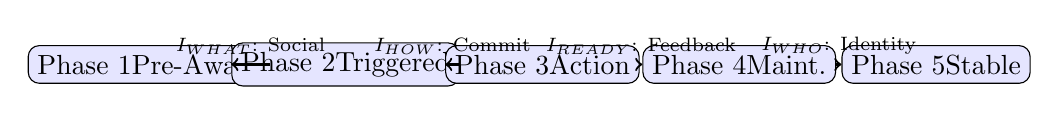
\begin{tikzpicture}[node distance=2.5cm, auto]
    \node[draw, rounded corners, fill=blue!10] (p1) {Phase 1\\Pre-Aware};
    \node[draw, rounded corners, fill=blue!10, right of=p1] (p2) {Phase 2\\Triggered};
    \node[draw, rounded corners, fill=blue!10, right of=p2] (p3) {Phase 3\\Action};
    \node[draw, rounded corners, fill=blue!10, right of=p3] (p4) {Phase 4\\Maint.};
    \node[draw, rounded corners, fill=blue!10, right of=p4] (p5) {Phase 5\\Stable};

    \draw[->, thick] (p1) -- node[above, font=\scriptsize] {$I_{\text{WHAT}}$: Social} (p2);
    \draw[->, thick] (p2) -- node[above, font=\scriptsize] {$I_{\text{HOW}}$: Commit} (p3);
    \draw[->, thick] (p3) -- node[above, font=\scriptsize] {$I_{\text{READY}}$: Feedback} (p4);
    \draw[->, thick] (p4) -- node[above, font=\scriptsize] {$I_{\text{WHO}}$: Identity} (p5);
\end{tikzpicture}
\end{center}


%%%%%%%%%%%%%%%%%%%%%%%%%%%%%%%%%%%%%%%%%%%%%%%%%%%%%%%%%%%%%%%%%%%%%%%%%%%%%%%
\section{Mismatch-Kosten: Was schiefgehen kann}
\label{sec:18-mismatch}
%%%%%%%%%%%%%%%%%%%%%%%%%%%%%%%%%%%%%%%%%%%%%%%%%%%%%%%%%%%%%%%%%%%%%%%%%%%%%%%

Phase-Intervention Misalignment verursacht substanzielle \textbf{Mismatch-Kosten}.

\subsection{Quantifizierung der Mismatch-Kosten}

\begin{definition}[Mismatch Cost]
\label{def:18-mismatch}
Die Mismatch-Kosten $\mathcal{L}_{mm}$ sind der Effektivitätsverlust durch falsche Phasenzuordnung:
\begin{equation}
\mathcal{L}_{mm}(t, \varphi, \varphi^*) = E_{\max} \cdot (\alpha_{t,\varphi^*} - \alpha_{t,\varphi})
\label{eq:18-mismatch-cost}
\end{equation}
wobei $\varphi^*$ die optimale Phase für Typ $t$ und $\varphi$ die tatsächliche Phase ist.
\end{definition}

\subsection{Typische Mismatch-Szenarien}

\begin{table}[htbp]
\centering
\caption{Häufige Mismatch-Szenarien und ihre Kosten}
\label{tab:18-mismatch-scenarios}
\renewcommand{\arraystretch}{1.3}
\small
\begin{tabular}{@{}llccc@{}}
\toprule
\textbf{Dominante $I_c$} & \textbf{Falsche Phase} & \textbf{$\alpha_{\text{falsch}}$} & \textbf{$\alpha_{\text{optimal}}$} & \textbf{Verlust} \\
\midrule
$I_{\text{HOW}}$ hoch (Commitment) & Pre-Awareness & 0.12 & 0.88 & 86\% \\
$I_{\text{AWARE}}$ hoch (Information) & Stable & 0.10 & 0.85 & 88\% \\
$I_{\text{WHO}}$ hoch (Identity) & Pre-Awareness & 0.18 & 0.90 & 80\% \\
$I_{\text{WHAT}}$ (Financial) & Pre-Awareness & 0.25 & 0.85 & 71\% \\
\bottomrule
\end{tabular}
\end{table}

\textbf{Kern-Einsicht:} Die falsche Intervention zur falschen Zeit verschwendet 70--90\% des Potentials.

\subsection{Sekundäre Mismatch-Kosten}

Über den direkten Effektivitätsverlust hinaus:
\begin{enumerate}
\item \textbf{Reaktanz:} Zu frühe Commitment-Aufforderung → Widerstand
\item \textbf{Desensibilisierung:} Wiederholte Information ohne Fortschritt → ``Tune out''
\item \textbf{Ressourcenverschwendung:} Budget für wirkungslose Maßnahmen verbraucht
\item \textbf{Opportunitätskosten:} Zeitfenster für effektive Intervention verpasst
\end{enumerate}


%%%%%%%%%%%%%%%%%%%%%%%%%%%%%%%%%%%%%%%%%%%%%%%%%%%%%%%%%%%%%%%%%%%%%%%%%%%%%%%
\section{Worked Examples}
\label{sec:18-examples}
%%%%%%%%%%%%%%%%%%%%%%%%%%%%%%%%%%%%%%%%%%%%%%%%%%%%%%%%%%%%%%%%%%%%%%%%%%%%%%%

\subsection{Beispiel 1: Thomas's vollständige Rauchentwöhnung}

\textbf{Kontext:} Thomas, 52, 30 Jahre Raucher, initial in Phase 1.

\begin{table}[htbp]
\centering
\caption{Journey-integrierte Interventions-Sequenz: Rauchentwöhnung}
\label{tab:18-example-thomas}
\renewcommand{\arraystretch}{1.3}
\small
\begin{tabular}{@{}cllllc@{}}
\toprule
\textbf{Woche} & \textbf{Phase} & \textbf{Intervention} & \textbf{Dominante $I_c$} & \textbf{$\pi$} & \textbf{$\alpha$} \\
\midrule
0--4 & Pre-Aware & Social Norm: ``70\% wollen aufh\"{o}ren'' & $I_{\text{WHAT}}$ (social) & $\pi_D$ & 0.75 \\
5--8 & Triggered & Quit-Date Commitment Card & $I_{\text{HOW}}$ & $\pi_E$ & 0.88 \\
9--16 & Action & Nikotinpflaster + Tracking-App & $I_{\text{READY}} + I_{\text{WHEN}}$ & $\pi_A$ & 0.90 \\
17--26 & Maintenance & Ex-Raucher Supportgruppe & $I_{\text{WHAT}}$ (social) & $\pi_A$ & 0.78 \\
27+ & Stable & ``Ich bin Nichtraucher''-Identit\"{a}t & $I_{\text{WHO}}$ & $\pi_S$ & 0.90 \\
\bottomrule
\end{tabular}
\end{table}

\textbf{Berechnung des Gesamt-Effekts:}
\begin{equation}
E_{\text{total}} = \prod_k \alpha_k = 0.75 \times 0.88 \times 0.90 \times 0.78 \times 0.90 = 0.42
\label{eq:18-thomas-effect}
\end{equation}

\textbf{Interpretation:} 42\% des theoretischen Maximums --- realistisch für komplexe Verhaltensänderung.

\subsection{Beispiel 2: Finanzielle Vorsorge bei Berufseinsteigern}

\textbf{Kontext:} Bank will Sparquote bei 25--30-Jährigen von 5\% auf 12\% erhöhen.

\textbf{Phase-Diagnose:} Zielgruppe primär in Phase 2 (Triggered) --- wissen, dass sie sparen sollten, tun es aber nicht.

\begin{table}[htbp]
\centering
\caption{Interventions-Sequenz: Finanzielle Vorsorge}
\label{tab:18-example-finance}
\renewcommand{\arraystretch}{1.3}
\small
\begin{tabular}{@{}llllc@{}}
\toprule
\textbf{Zeitraum} & \textbf{Phase} & \textbf{Intervention} & \textbf{Mechanismus} & \textbf{$\alpha$} \\
\midrule
Monat 1 & Triggered & Save More Tomorrow™ & Auto-Escalation Commitment & 0.88 \\
Monat 2--6 & Action & Spar-Fortschritts-App & Feedback + Gamification & 0.88 \\
Monat 7--12 & Maintenance & Peer-Vergleich: ``Du sparst mehr als 65\%'' & Social Norm & 0.78 \\
Ab Jahr 2 & Stable & ``Ich bin ein Sparer''-Badge & Identity Reinforcement & 0.90 \\
\bottomrule
\end{tabular}
\end{table}

\textbf{Erwartete Sparquoten-Erhöhung:}
\begin{equation}
\Delta \text{Sparquote} = (12\% - 5\%) \times 0.88 \times 0.88 \times 0.78 = +4.2\%
\label{eq:18-finance-effect}
\end{equation}

Realistische Erwartung: Sparquote steigt von 5\% auf 9.2\% (nicht 12\%, da nicht alle reagieren).

\subsection{Beispiel 3: Corporate Wellness (Kontrast: Mit vs.\ Ohne Journey-Integration)}

\textbf{Kontext:} Unternehmen mit 1,000 Mitarbeitern, Ziel: Mehr Bewegung.

\textbf{Ansatz A: Ohne Journey-Integration}
\begin{itemize}
\item Alle bekommen Fitness-Tracker + Wettbewerb ($I_{\text{READY}} + I_{\text{WHAT}}$ social)
\item Problem: 40\% sind Pre-Aware → $\alpha = 0.20$
\item Durchschnittliche Effektivität: $0.4 \times 0.20 + 0.6 \times 0.70 = 0.50$
\end{itemize}

\textbf{Ansatz B: Mit Journey-Integration}
\begin{itemize}
\item Phase 1 (40\%): Gesundheits-Assessment + Personalisierte Risiko-Info ($I_{\text{AWARE}}$ hoch) $\rightarrow$ $\alpha = 0.85$
\item Phase 2+ (60\%): Fitness-Tracker + Wettbewerb ($I_{\text{READY}} + I_{\text{WHAT}}$ social) $\rightarrow$ $\alpha = 0.80$
\item Durchschnittliche Effektivität: $0.4 \times 0.85 + 0.6 \times 0.80 = 0.82$
\end{itemize}

\textbf{Effizienzgewinn durch Journey-Integration:} $\frac{0.82}{0.50} = 1.64\times$ (+64\%)


%%%%%%%%%%%%%%%%%%%%%%%%%%%%%%%%%%%%%%%%%%%%%%%%%%%%%%%%%%%%%%%%%%%%%%%%%%%%%%%
\section{Summary}
\label{sec:18-summary}
%%%%%%%%%%%%%%%%%%%%%%%%%%%%%%%%%%%%%%%%%%%%%%%%%%%%%%%%%%%%%%%%%%%%%%%%%%%%%%%

\begin{tcolorbox}[colback=green!10!white, colframe=green!75!black,
    title=Key Points (Emergent Temporal Theory)]

\textbf{Core Message:} Journey-Position und Wirkungs-Horizont \textbf{emergieren} aus den fundamentalen Vektoren---sie sind keine ontologischen Kategorien.

\textbf{Key Takeaways:}
\begin{enumerate}
\item \textbf{EIT-4 (Journey-Emergenz):} $\varphi = h(\vec{S}_0)$ --- Journey-Position emergiert aus 10C Status Quo
\item \textbf{EIT-5 (Horizont-Emergenz):} $\tau = g(\vec{I})$ --- Wirkungs-Horizont emergiert aus Interventionsvektor
\item \textbf{Kontinuierliche Affinity:} $\alpha(\vec{I}, \vec{S}_0)$ als Feld über dem Produktraum
\item \textbf{K*-Integration (EIT-EMP-2):} Phase-Affinity $\alpha$ bestimmt Stage-Faktor $f_S$ in $K^*$
\item \textbf{Mismatch-Kosten:} Falsche Phase = 70--90\% Effektivitätsverlust; EMERGE warnt bei $\alpha < 0.3$
\item \textbf{Effizienzgewinn:} Journey-Integration steigert Effektivität um 50--70\%
\end{enumerate}

\textbf{Weiter zu:} Chapter 11 (EMERGE-Algorithmus für $K^*$), Kapitel 20 (Portfolios mit C1-C7).

\end{tcolorbox}

%------------------------------------------------------------------------------
\paragraph{Formal Details.}
Die vollständige formale Behandlung findet sich in:
\begin{itemize}[nosep]
\item Appendix STA (CORE-STAGE) --- Axiome STA-1 bis STA-4, $S(t)$ Progression Function
\item Appendix HHH (METHOD-TOOLKIT) --- Theorem HHH-T5 (Phase Emergence), F6 und F14 Felder
\item Appendix PAP (FORMAL-EQUILIBRIA) --- Übergangs-Dynamiken, Tipping Points
\item Appendix EST (CORE-WHERE) --- Literatur-basierte $\alpha$-Schätzungen mit Quellen
\end{itemize}

%------------------------------------------------------------------------------
\paragraph{What Comes Next.}
\begin{itemize}[nosep]
\item \textbf{Kapitel 11 §11.20:} EMERGE-Algorithmus --- wie $\alpha$ in den Stage-Faktor $f_S$ von $K^*$ eingeht
\item \textbf{Kapitel 19:} Segment-Dimension --- Segment-Multiplier $\sigma_s$ für Targeting
\item \textbf{Kapitel 20:} Portfolios mit Constraints C1-C7 --- inkl. Phase-Constraint (C3: Timing)
\end{itemize}


% -----------------------------------------------------------------------------
% READING PATH BOX
% -----------------------------------------------------------------------------

\begin{tcolorbox}[colback=gray!5!white, colframe=gray!75!black,
    title=Empfohlene Lesepfade]

\textbf{Abgeschlossen:} Chapter 18 (Journey-Integrated Interventions)

\textbf{Sie verstehen jetzt:}
\begin{itemize}[nosep]
\item Wie die Phase-Type Affinity Matrix $\alpha_{t,\varphi}$ funktioniert
\item Warum Diagnosis-First essentiell ist
\item Wie Path Functions den Journey strukturieren
\item Welche Mismatch-Kosten entstehen
\end{itemize}

\textbf{Nächste Schritte:}
\begin{itemize}[nosep]
\item \textbf{Kapitel 11 §11.20}: EMERGE-Algorithmus --- $\alpha \to f_S \to K^*$ (EIT-EMP-2)
\item \textbf{Kapitel 19}: Segment-Specific Interventions --- $\sigma_s$ für Targeting
\item \textbf{Kapitel 20}: Portfolios mit C1-C7 --- inkl.\ Timing-Constraint (C3) und K*-Constraint (C7)
\end{itemize}

\textbf{Für Vertiefung:} Appendix STA (Journey-Axiome), Appendix IE (EMERGE-SPEC), Appendix HHH (F6, F14)
\end{tcolorbox}


% =============================================================================
% POLICY IMPLICATIONS
% =============================================================================

\section*{Policy Implications}

\begin{enumerate}
\item \textbf{Für Gesundheitswesen:} Präventionsprogramme müssen Journey-Phase diagnostizieren \textit{bevor} Intervention gewählt wird. Universelle Kampagnen (``One-size-fits-all'') verschwenden 50--70\% des Potentials.

\item \textbf{Für HR/Change Management:} Organisationale Veränderungsprogramme sollten Mitarbeiter nach Journey-Phase segmentieren. Resistance gegen Change ist oft Mismatch zwischen Intervention und Phase.

\item \textbf{Für Finanzdienstleister:} Altersvorsorge-Kampagnen sollten mit Staging beginnen. Save More Tomorrow™ funktioniert nur bei Triggered-Kunden; Pre-Aware brauchen erst Awareness-Interventionen.

\item \textbf{Für Policy-Maker:} Langfristige Verhaltensänderung erfordert Journey-begleitende Interventions-\textit{Sequenzen}, nicht einmalige Maßnahmen. Budget sollte über Phasen verteilt werden.
\end{enumerate}


% =============================================================================
% END OF CHAPTER 18
% =============================================================================
